\section{Discriminator approximation of total correlation} \label{sec:disc_approx}
This section describes how density ratio estimation is implemented to train the FFVAE encoder.
We follow the approach of \citet{kim2018disentangling}.
\paragraph{Generating Samples}
The binary classifier adversary seeks to discriminate between
\begin{itemize}
    \item $[z,b] \sim q(z,b)$, ``true'' samples from the aggregate posterior; and
    \item $[z',b'] \sim q(z)\prod_j q(b_j)$, ``fake'' samples from the product of the marginal over $z$ and the marginals over each $b_j$.
\end{itemize}
At train time, after splitting the latent code $[z^i,b^i]$ of the $i$-example along the dimensions of $b$ as $[z^i, b_0^i ... b_j^i]$, the minibatch index order for each subspace is then randomized, simulating samples from the product of the marginals; these dimension-shuffled samples retain the same marginal statistics as ``real'' (unshuffled) samples, but with joint statistics between the subspaces broken.
The overall minibatch of encoder outputs contains twice as many examples as the original image minibatch, and comprises equal number of ``real'' and ``fake'' samples.

As we describe below, the encoder output minibatch is used as training data for the adversary, and the error is backpropagated to the encoder weights so the encoder can better fool the adversary.
 If a strong adversary can do no better than random chance, then the desired independence property has been achieved.

\paragraph{Discriminator Approximation}
Here we summarize the the approximation of the $D_{KL}(q(z,b)||q(z)\prod_{j} q(b_j))$ term from equation \ref{eq:ffvae}.
Let $u \in \{0, 1\}$ be an indicator variable with $u=1$ indicating $[z,b] \sim q(z,b)$ comes from a minibatch of ``real'' encoder distributions, while $u=1$ indicating $[z',b'] \sim q(z)\prod_j(b_j)$ is drawn from a ``fake'' minibatch of shuffled samples, i.e., is drawn from the product of the marginals of the aggregate posterior.
The discriminator network outputs the probability that vector $[z,b]$ is a ``real'' sample, i.e., 
$d(u|z,b)=\text{Bernoulli}(u|\sigma(\theta_{d}(z,b))$ 
where $\theta_d(z,b)$ 
is the discriminator and $\sigma$ is the sigmoid function.
If the discriminator is well-trained to distinguish between ``real'' and ``fake'' samples then we have 
\begin{align}
    \log d(u=1|z,b) - \log d(u=0|z,b) &\approx \nonumber \\
    \log q(z,b) - \log q(z)\prod_j q(b_j).
\end{align}
We can substitute this into the KL divergence as 
\begin{align}
    &D_{KL}(q(z,b)||q(z)\prod_{j} q(b_j)) = \nonumber \\
    &\quad\quad \E_{q(z,b)}[ \log q(z,b) - \log q(z)\prod_j q(b_j) ] \approx \nonumber \\
    &\quad\quad \E_{q(z,b)}[ \log d(u=1|z,b) - \log d(u=0|z,b)].
\end{align}

Meanwhile the discriminator is trained by minimizing the standard cross entropy loss
\begin{align}
    L_{\text{Disc}}(d) &= \E_{z,b\sim q(z,b)} [\log d(u=1|z,b)] \nonumber \\
    &\quad\quad + \E_{z',b'\sim q(z)\prod_j q(b_j)} [\log ( 1 - d(u=0|z',b') )],
\end{align}
w.r.t. the parameters of $d(u|z,b)$.
This ensures that the discriminator output $\theta_d(z,b)$ is a calibrated approximation of the log density $\log\frac{q(z,b)}{q(z)\prod_j q(b_j)}$.

$L_{\text{Disc}}(d)$ and $L_{\text{FFVAE}}(p,q)$ (Equation \ref{eq:ffvae}) are then optimized in a min-max fashion.
In our experiments we found that single-step alternating updates using optimizers with the same settings sufficed for stable optimization.

\section{DSpritesUnfair Generation} \label{sec:dsprites-generation}
The original DSprites dataset has six ground truth factors of variation (FOV): 
\begin{itemize}
    \item Color: white
    \item Shape: square, ellipse, heart
    \item Scale: 6 values linearly spaced in $[0.5, 1]$
    \item Orientation: 40 values in $[0, 2\pi]$
    \item XPosition: 32 values in $[0, 1]$
    \item YPosition: 32 values in $[0, 1]$
\end{itemize}

In the original dataset the joint distribution over all FOV factorized; each FOV was considered independent.
In our dataset, we instead sample such that the FOVs Shape and X-position correlate.
We associate an index with each possible value of each attribute, and then sample a (Shape, X-position) pair with probability proportional to $(\frac{i_S}{n_S})^{q_S} + (\frac{i_X}{n_X})^{q_X}$, where $i, n, q$ are the indices, total number of options, and a real number for each of Shape and X-position ($S, X$ respectively).
We use $q_S = 1, q_X = 3$. 
All other attributes are sampled uniformly, as in the standard version of DSprites.

We binarized the factors of variation by using the boolean outputs of the following operations:
\begin{itemize}
    \item Color $\geq 1$
    \item Shape $\geq 1$
    \item Scale $\geq 3$
    \item Rotation $\geq 20$
    \item XPosition $\geq 16$
    \item YPosition $\geq 16$
\end{itemize}

\section{DSprites Architectures}\label{sec:archs}
The architectures for the convolutional encoder $q(z,b|x)$, decoder $q(x|z,b)$, and FFVAE discriminator are specified as follows.
{\tiny

\begin{verbatim}
import torch
from torch import nn

class Resize(torch.nn.Module):
    def __init__(self, size):
        super(Resize, self).__init__()
        self.size = size

    def forward(self, tensor):
        return tensor.view(self.size)

class ConvEncoder(nn.Module):
    def __init__(self, im_shape=[64, 64], latent_dim=10, n_chan=1):
        super(ConvEncoder, self).__init__()

        self.f = nn.Sequential(
            Resize((-1,n_chan,im_shape[0],im_shape[1])),
            nn.Conv2d(n_chan, 32, 4, 2, 1),
            nn.ReLU(True),
            nn.Conv2d(32, 32, 4, 2, 1),
            nn.ReLU(True),
            nn.Conv2d(32, 64, 4, 2, 1),
            nn.ReLU(True),
            nn.Conv2d(64, 64, 4, 2, 1),
            nn.ReLU(True),
            Resize((-1,1024)),
            nn.Linear(1024, 128),
            nn.ReLU(True),
            nn.Linear(128, 2*latent_dim)
            )
        self.im_shape = im_shape
        self.latent_dim = latent_dim

    def forward(self, x):
        mu_and_logvar = self.f(x)
        mu = mu_and_logvar[:, :self.latent_dim]
        logvar = mu_and_logvar[:, self.latent_dim:]
        return mu, logvar

class ConvDecoder(nn.Module):
    def __init__(self, im_shape=[64, 64], latent_dim=10, n_chan=1):
        super(ConvDecoder, self).__init__()

        self.g = nn.Sequential(
            nn.Linear(latent_dim, 128),
            nn.ReLU(True),
            nn.Linear(128, 1024),
            nn.ReLU(True),
            Resize((-1,64,4,4)),
            nn.ConvTranspose2d(64, 64, 4, 2, 1),
            nn.ReLU(True),
            nn.ConvTranspose2d(64, 32, 4, 2, 1),
            nn.ReLU(True),
            nn.ConvTranspose2d(32, 32, 4, 2, 1),
            nn.ReLU(True),
            nn.ConvTranspose2d(32, n_chan, 4, 2, 1),
            )

    def forward(self, z):
        x = self.g(z)
        return x.squeeze()

class Discriminator(nn.Module):
    def __init__(self, n):
        super(Discriminator, self).__init__()
        self.model = nn.Sequential(
            nn.Linear(n, 1000),
            nn.LeakyReLU(0.2, inplace=True),
            nn.Linear(1000, 1000),
            nn.LeakyReLU(0.2, inplace=True),
            nn.Linear(1000, 1000),
            nn.LeakyReLU(0.2, inplace=True),
            nn.Linear(1000, 1000),
            nn.LeakyReLU(0.2, inplace=True),
            nn.Linear(1000, 1000),
            nn.LeakyReLU(0.2, inplace=True),
            nn.Linear(1000, 2),
            )
        selftmax = nn.Softmax(dim=1)

    def forward(self, zb):
        logits = self.model(zb)
        probs = nn.Softmax(dim=1)(logits)
        return logits, probs
\end{verbatim}
}

\section{DSpritesUnfair Training Details}\label{sec:dsprites-training-details}
All network parameters were optimized using the Adam \citep{kingma2014adam}, with learning rate 0.001.
Architectures are specified in Appendix \ref{sec:archs}.
Our encoders trained $3 \times 10^5$ iterations with minibatch size 64 (as in \citet{kim2018disentangling}).
Our MLP classifier has two hidden layers with 128 units each, and is trained with patience of 5 epochs on validation loss.

\section{Mutual Information Gap} \label{sec:mig}
\paragraph{Evaluation Criteria}
Here we analyze the encoder mutual information in the synthetic setting of the DSpritesUnfair dataset, where we know the ground truth factors of variation.
In Fig. \ref{fig:dsprites-mig}, we calculate the \textit{Mutual Information Gap (MIG)} \citep{chen2018isolating} of FFVAE across various hyperparameter settings.
With $J$ latent variables $z_j$ and $K$ factors of variation $v_k$, MIG is defined as 
\begin{equation}
    \frac{1}{K} \sum_{k=1}^{K} \frac{1}{H(v_k)} (MI (z_{j_k}; v_k) - \max_{j \neq j_k} MI (z_j; v_k))
\end{equation}
where $j_k = \underset{j}{\argmax} MI (z_j; v_k)$, $MI(\cdot; \cdot)$ denotes mutual information, and $K$ is the number of factors of variation.
Note that we can only compute this metric in the synthetic setting where the ground truth factors of variation are known.
MIG measures the difference between the latent variables which have the highest and second-highest $MI$ with each factor of variation, rewarding models which allocate one latent variable to each factor of variation.
We test our disentanglement by training our models on a biased version of DSprites, and testing on a balanced version (similar to the ``skewed'' data in \citet{chen2018isolating}).
This allows us to separate out two sources of correlation --- the correlation existing across the data, and the correlation in the model's learned representation.

\paragraph{Results}
\begin{figure}[ht!]
%
% \begin{center}
% \centering
\begin{subfigure}[t]{0.23\textwidth}
% \centering
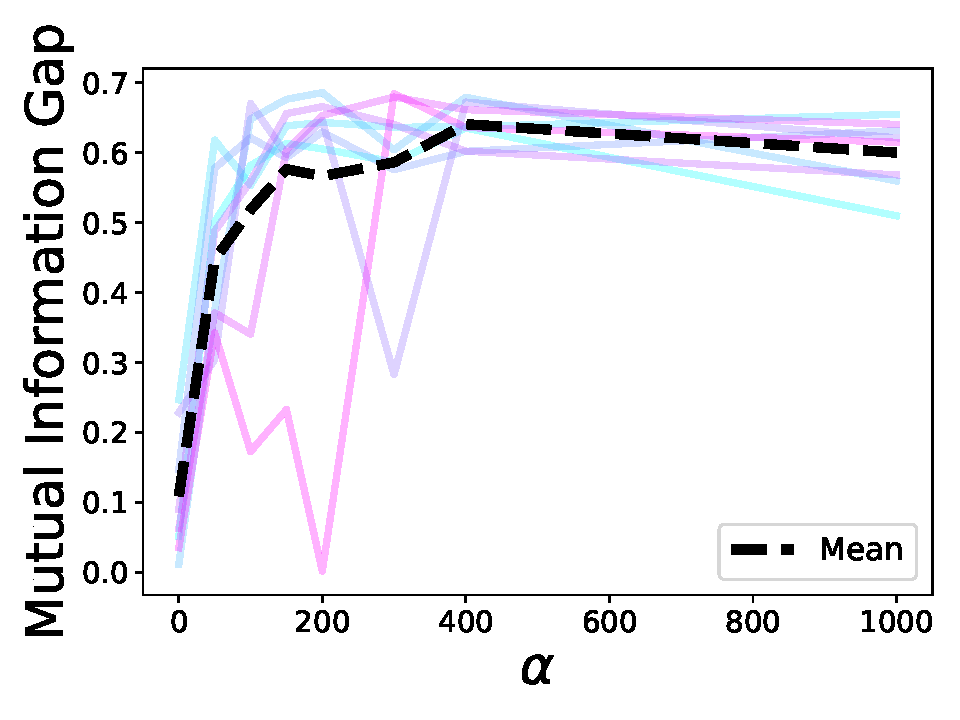
\includegraphics[width=\textwidth]{mig_beta_sens_gamma_lines.pdf}
\caption{Color is $\gamma$, brighter colours $\longrightarrow$ higher values}
\label{fig:dsprites-mig-lines}
\end{subfigure}
%
\hfill
%
\begin{subfigure}[t]{0.23\textwidth}
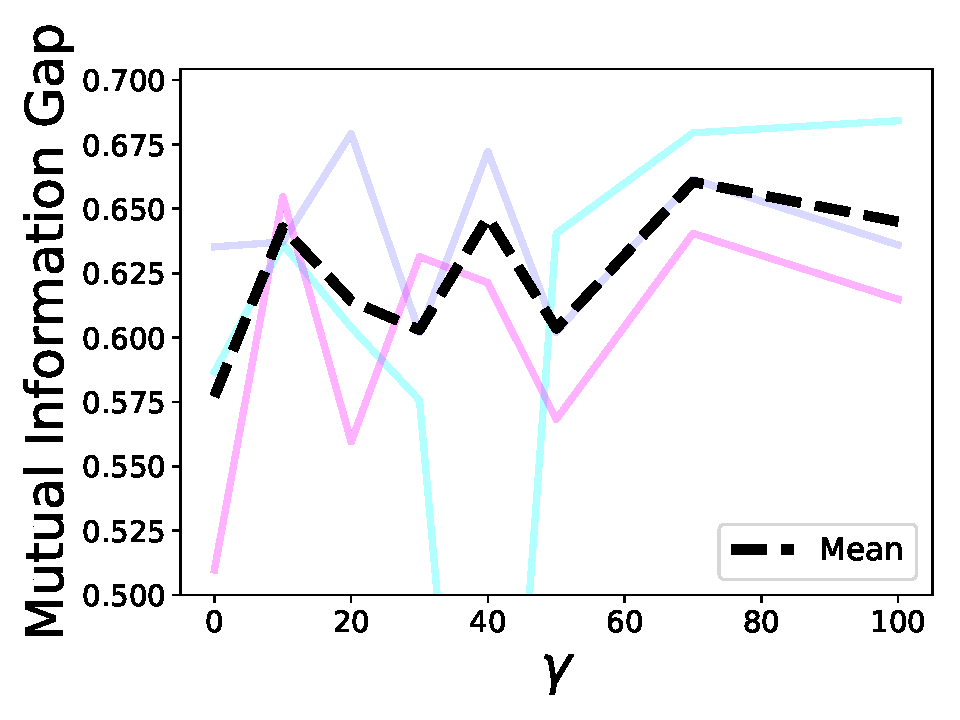
\includegraphics[width=\textwidth]{mig_gamma_beta_sens_high_lines.pdf}
\caption{Colour is $\alpha$, brighter colors $\longrightarrow$ higher values}
\label{fig:dsprites-mig-lines-high-alpha}
\end{subfigure}


\caption{
    Mutual Information Gap (MIG) for various $(\alpha, \gamma)$ settings of the FFVAE. 
    In Fig. \ref{fig:dsprites-mig-lines}, each line is a different value of
    $\gamma \in [10, 20, 30, 40, 50, 70, 100]$, with brighter colors indicating larger values of $\gamma$.
    In Fig. \ref{fig:dsprites-mig-lines-high-alpha}, each line is a different value of
    $\alpha \in [300, 400, 1000]$, with brighter colors indicating larger values of $\alpha$.
    Models trained on DspritesUnfair, MIG calculated on Dsprites.
    Higher MIG is better.
    Black dashed line indicates mean (with outliers excluded).
    $\alpha = 0$ is equivalent to the FactorVAE.
    }
    \label{fig:dsprites-mig}
% \end{center}
% \vskip -0.2in
\end{figure}


In Fig. \ref{fig:dsprites-mig-lines}, we show that MIG increases with $\alpha$, providing more evidence that the supervised structure of the FFVAE can create disentanglement.
This improvement holds across values of $\gamma$, except for some training instability for the highest values of $\gamma$.
It is harder to assess the relationship between $\gamma$ and MIG, due to increased instability in training when $\gamma$ is large and $\alpha$ is small.
However, in Fig. \ref{fig:dsprites-mig-lines-high-alpha}, we look only at $\alpha \geq 300$, and note that in this range, MIG improves as $\gamma$ increases.
See Appendix \ref{sec:mig} for more details.

\begin{figure}[ht!]
%
% \begin{center}
% \centering
\begin{subfigure}[t]{0.23\textwidth}
% \centering
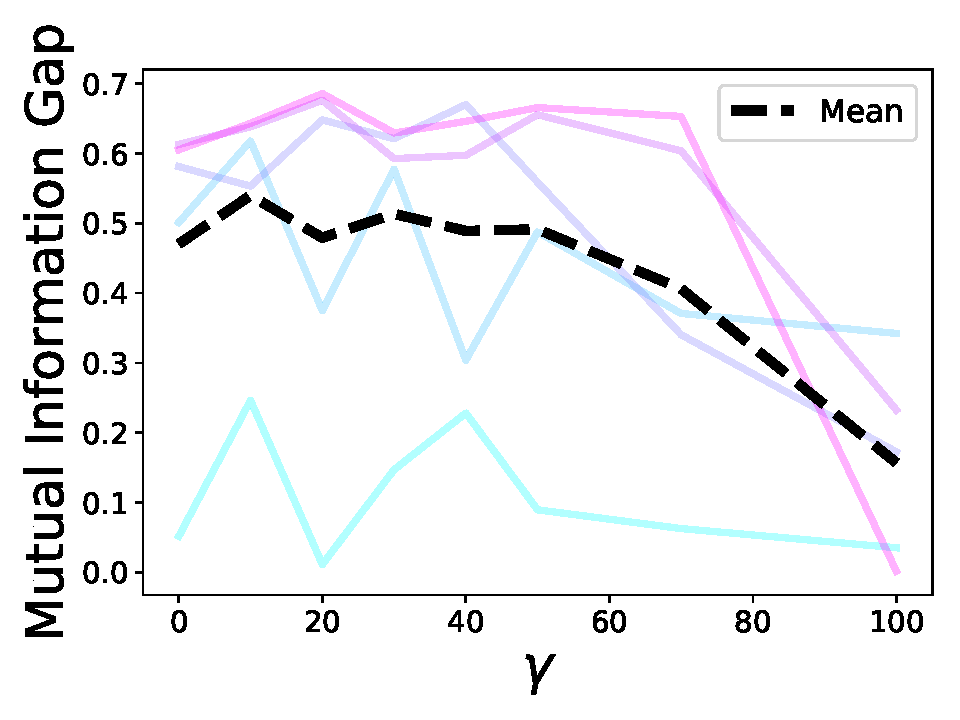
\includegraphics[width=\textwidth]{mig_gamma_beta_sens_low_lines.pdf}
\caption{Colour is $\alpha$}
\label{fig:dsprites-mig-lines-low-alpha}
\end{subfigure}
%
\hfill
%
\begin{subfigure}[t]{0.23\textwidth}
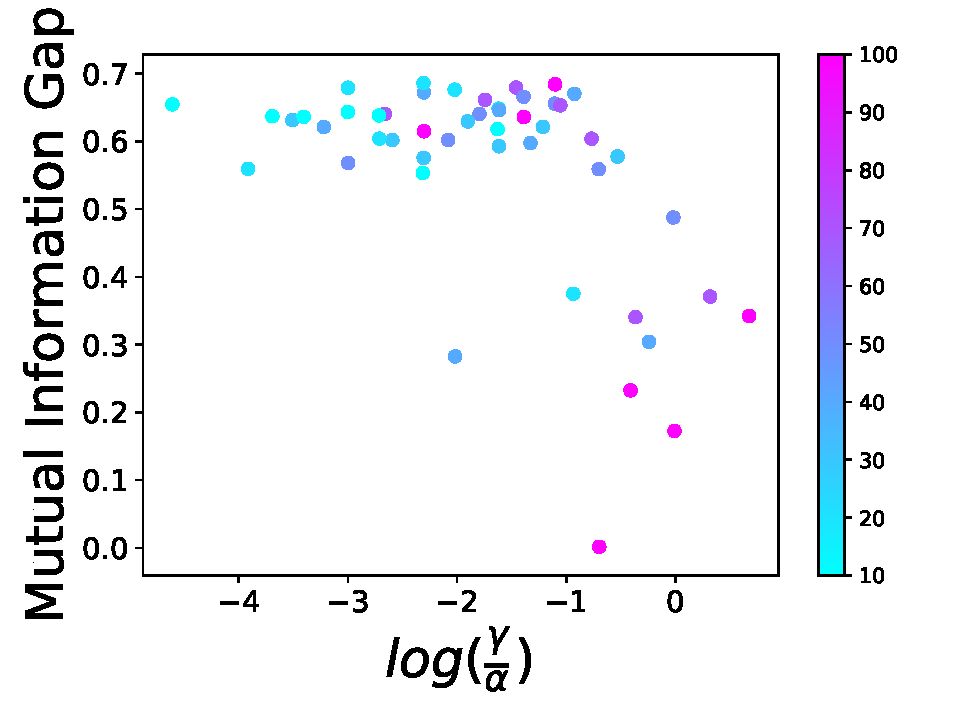
\includegraphics[width=\textwidth]{mig_gamma_betasens_ratio.pdf}
\caption{Colour is $\gamma$}
\label{fig:dsprites-mig-ratio}
\end{subfigure}


\caption{
    Mutual Information Gap (MIG) for various $(\alpha, \gamma)$ settings of the FFVAE. 
    In Fig. \ref{fig:dsprites-mig-lines-low-alpha}, each line is a different value of
    $\alpha \in [0, 50, 100, 150, 200]$, with brighter colours indicating larger values of $\alpha$.
    In Fig. \ref{fig:dsprites-mig-ratio}, all combinations with $\alpha, \gamma > 0$ are shown.
    Models trained on DspritesUnfair, MIG calculated on Dsprites.
    Higher MIG is better.
    Black dashed line indicates mean (outliers excluded).
    $\alpha = 0$ is equivalent to the FactorVAE.
    }
    \label{fig:dsprites-mig-appendix}
% \end{center}
% \vskip -0.2in
\end{figure}


In Fig. \ref{fig:dsprites-mig-lines-low-alpha}, we show that for low values of $\alpha$, increasing $\gamma$ leads to worse MIG, likely due to increased training instability.
This is in contrast to Fig. \ref{fig:dsprites-mig-lines-high-alpha}, which suggests that for high enough $\alpha$, increasing $\gamma$ can improve MIG.
This leads us to believe that $\alpha$ and $\gamma$ have a complex relationship with respect to disentanglement and MIG.

To better understand the relationship between these two hyperparameters, we examine how MIG varies with the ratio $\frac{\gamma}{\alpha}$ in Fig. \ref{fig:dsprites-mig-ratio}.
In We find that in general, a higher ratio yields lower MIG, but that the highest MIGs are around $\log\frac{\gamma}{\alpha} = -2$, with a slight tailing off for smaller ratios.
This indicates there is a dependent relationship between the values of $\gamma$ and $\alpha$.

\paragraph{Discussion}
What does it mean for our model to demonstrate disentanglement on test data drawn from a new distribution?
For interpretation, we can look to the causal inference literature, where one goal is to produce models that are robust to certain interventions in the data generating process \citep{rothlenhauser2018anchor}.
We can interpret Figure \ref{fig:dsprites-mig} as evidence that our learned representations are (at least partially) invariant to \textit{interventions} on $a$.
This property relates to counterfactual fairness, which requires that models be robust with respect to counterfactuals along $a$ \citep{kusner2017counterfactual}.

